\batchmode
\documentclass[11pt,a4paper]{article}
\RequirePackage{ifthen}




\usepackage[french]{babel}
\usepackage{pierre}
\usepackage{graphicx}
\usepackage{float}
\usepackage{amssymb}


\title{\textbf{Petite �tude des fractions continues et leur application � l'�quation de Pell}}
\author{\textbf{P. Paquay, \textsl{HEL - D�partement p�dagogique}}}
\date{}




\usepackage[dvips]{color}


\pagecolor[gray]{.7}

\usepackage[latin1]{inputenc}



\makeatletter

\makeatletter
\count@=\the\catcode`\_ \catcode`\_=8 
\newenvironment{tex2html_wrap}{}{}%
\catcode`\<=12\catcode`\_=\count@
\newcommand{\providedcommand}[1]{\expandafter\providecommand\csname #1\endcsname}%
\newcommand{\renewedcommand}[1]{\expandafter\providecommand\csname #1\endcsname{}%
  \expandafter\renewcommand\csname #1\endcsname}%
\newcommand{\newedenvironment}[1]{\newenvironment{#1}{}{}\renewenvironment{#1}}%
\let\newedcommand\renewedcommand
\let\renewedenvironment\newedenvironment
\makeatother
\let\mathon=$
\let\mathoff=$
\ifx\AtBeginDocument\undefined \newcommand{\AtBeginDocument}[1]{}\fi
\newbox\sizebox
\setlength{\hoffset}{0pt}\setlength{\voffset}{0pt}
\addtolength{\textheight}{\footskip}\setlength{\footskip}{0pt}
\addtolength{\textheight}{\topmargin}\setlength{\topmargin}{0pt}
\addtolength{\textheight}{\headheight}\setlength{\headheight}{0pt}
\addtolength{\textheight}{\headsep}\setlength{\headsep}{0pt}
\setlength{\textwidth}{349pt}
\newwrite\lthtmlwrite
\makeatletter
\let\realnormalsize=\normalsize
\global\topskip=2sp
\def\preveqno{}\let\real@float=\@float \let\realend@float=\end@float
\def\@float{\let\@savefreelist\@freelist\real@float}
\def\liih@math{\ifmmode$\else\bad@math\fi}
\def\end@float{\realend@float\global\let\@freelist\@savefreelist}
\let\real@dbflt=\@dbflt \let\end@dblfloat=\end@float
\let\@largefloatcheck=\relax
\let\if@boxedmulticols=\iftrue
\def\@dbflt{\let\@savefreelist\@freelist\real@dbflt}
\def\adjustnormalsize{\def\normalsize{\mathsurround=0pt \realnormalsize
 \parindent=0pt\abovedisplayskip=0pt\belowdisplayskip=0pt}%
 \def\phantompar{\csname par\endcsname}\normalsize}%
\def\lthtmltypeout#1{{\let\protect\string \immediate\write\lthtmlwrite{#1}}}%
\newcommand\lthtmlhboxmathA{\adjustnormalsize\setbox\sizebox=\hbox\bgroup\kern.05em }%
\newcommand\lthtmlhboxmathB{\adjustnormalsize\setbox\sizebox=\hbox to\hsize\bgroup\hfill }%
\newcommand\lthtmlvboxmathA{\adjustnormalsize\setbox\sizebox=\vbox\bgroup %
 \let\ifinner=\iffalse \let\)\liih@math }%
\newcommand\lthtmlboxmathZ{\@next\next\@currlist{}{\def\next{\voidb@x}}%
 \expandafter\box\next\egroup}%
\newcommand\lthtmlmathtype[1]{\gdef\lthtmlmathenv{#1}}%
\newcommand\lthtmllogmath{\dimen0\ht\sizebox \advance\dimen0\dp\sizebox
  \ifdim\dimen0>.95\vsize
   \lthtmltypeout{%
*** image for \lthtmlmathenv\space is too tall at \the\dimen0, reducing to .95 vsize ***}%
   \ht\sizebox.95\vsize \dp\sizebox\z@ \fi
  \lthtmltypeout{l2hSize %
:\lthtmlmathenv:\the\ht\sizebox::\the\dp\sizebox::\the\wd\sizebox.\preveqno}}%
\newcommand\lthtmlfigureA[1]{\let\@savefreelist\@freelist
       \lthtmlmathtype{#1}\lthtmlvboxmathA}%
\newcommand\lthtmlpictureA{\bgroup\catcode`\_=8 \lthtmlpictureB}%
\newcommand\lthtmlpictureB[1]{\lthtmlmathtype{#1}\egroup
       \let\@savefreelist\@freelist \lthtmlhboxmathB}%
\newcommand\lthtmlpictureZ[1]{\hfill\lthtmlfigureZ}%
\newcommand\lthtmlfigureZ{\lthtmlboxmathZ\lthtmllogmath\copy\sizebox
       \global\let\@freelist\@savefreelist}%
\newcommand\lthtmldisplayA{\bgroup\catcode`\_=8 \lthtmldisplayAi}%
\newcommand\lthtmldisplayAi[1]{\lthtmlmathtype{#1}\egroup\lthtmlvboxmathA}%
\newcommand\lthtmldisplayB[1]{\edef\preveqno{(\theequation)}%
  \lthtmldisplayA{#1}\let\@eqnnum\relax}%
\newcommand\lthtmldisplayZ{\lthtmlboxmathZ\lthtmllogmath\lthtmlsetmath}%
\newcommand\lthtmlinlinemathA{\bgroup\catcode`\_=8 \lthtmlinlinemathB}
\newcommand\lthtmlinlinemathB[1]{\lthtmlmathtype{#1}\egroup\lthtmlhboxmathA
  \vrule height1.5ex width0pt }%
\newcommand\lthtmlinlineA{\bgroup\catcode`\_=8 \lthtmlinlineB}%
\newcommand\lthtmlinlineB[1]{\lthtmlmathtype{#1}\egroup\lthtmlhboxmathA}%
\newcommand\lthtmlinlineZ{\egroup\expandafter\ifdim\dp\sizebox>0pt %
  \expandafter\centerinlinemath\fi\lthtmllogmath\lthtmlsetinline}
\newcommand\lthtmlinlinemathZ{\egroup\expandafter\ifdim\dp\sizebox>0pt %
  \expandafter\centerinlinemath\fi\lthtmllogmath\lthtmlsetmath}
\newcommand\lthtmlindisplaymathZ{\egroup %
  \centerinlinemath\lthtmllogmath\lthtmlsetmath}
\def\lthtmlsetinline{\hbox{\vrule width.1em \vtop{\vbox{%
  \kern.1em\copy\sizebox}\ifdim\dp\sizebox>0pt\kern.1em\else\kern.3pt\fi
  \ifdim\hsize>\wd\sizebox \hrule depth1pt\fi}}}
\def\lthtmlsetmath{\hbox{\vrule width.1em\kern-.05em\vtop{\vbox{%
  \kern.1em\kern0.8 pt\hbox{\hglue.17em\copy\sizebox\hglue0.8 pt}}\kern.3pt%
  \ifdim\dp\sizebox>0pt\kern.1em\fi \kern0.8 pt%
  \ifdim\hsize>\wd\sizebox \hrule depth1pt\fi}}}
\def\centerinlinemath{%
  \dimen1=\ifdim\ht\sizebox<\dp\sizebox \dp\sizebox\else\ht\sizebox\fi
  \advance\dimen1by.5pt \vrule width0pt height\dimen1 depth\dimen1 
 \dp\sizebox=\dimen1\ht\sizebox=\dimen1\relax}

\def\lthtmlcheckvsize{\ifdim\ht\sizebox<\vsize 
  \ifdim\wd\sizebox<\hsize\expandafter\hfill\fi \expandafter\vfill
  \else\expandafter\vss\fi}%
\providecommand{\selectlanguage}[1]{}%
\makeatletter \tracingstats = 1 


\begin{document}
\pagestyle{empty}\thispagestyle{empty}\lthtmltypeout{}%
\lthtmltypeout{latex2htmlLength hsize=\the\hsize}\lthtmltypeout{}%
\lthtmltypeout{latex2htmlLength vsize=\the\vsize}\lthtmltypeout{}%
\lthtmltypeout{latex2htmlLength hoffset=\the\hoffset}\lthtmltypeout{}%
\lthtmltypeout{latex2htmlLength voffset=\the\voffset}\lthtmltypeout{}%
\lthtmltypeout{latex2htmlLength topmargin=\the\topmargin}\lthtmltypeout{}%
\lthtmltypeout{latex2htmlLength topskip=\the\topskip}\lthtmltypeout{}%
\lthtmltypeout{latex2htmlLength headheight=\the\headheight}\lthtmltypeout{}%
\lthtmltypeout{latex2htmlLength headsep=\the\headsep}\lthtmltypeout{}%
\lthtmltypeout{latex2htmlLength parskip=\the\parskip}\lthtmltypeout{}%
\lthtmltypeout{latex2htmlLength oddsidemargin=\the\oddsidemargin}\lthtmltypeout{}%
\makeatletter
\if@twoside\lthtmltypeout{latex2htmlLength evensidemargin=\the\evensidemargin}%
\else\lthtmltypeout{latex2htmlLength evensidemargin=\the\oddsidemargin}\fi%
\lthtmltypeout{}%
\makeatother
\setcounter{page}{1}
\onecolumn

% !!! IMAGES START HERE !!!

\stepcounter{section}
{\newpage\clearpage
\lthtmlinlinemathA{tex2html_wrap_inline645}%
$x^2 - dy^2 = 1$%
\lthtmlinlinemathZ
\lthtmlcheckvsize\clearpage}

\stepcounter{section}
{\newpage\clearpage
\lthtmlinlinemathA{tex2html_wrap_inline647}%
$16$%
\lthtmlinlinemathZ
\lthtmlcheckvsize\clearpage}

{\newpage\clearpage
\lthtmlinlinemathA{tex2html_wrap_inline649}%
$9$%
\lthtmlinlinemathZ
\lthtmlcheckvsize\clearpage}

{\newpage\clearpage
\lthtmlpictureA{tex2html_wrap1401}%
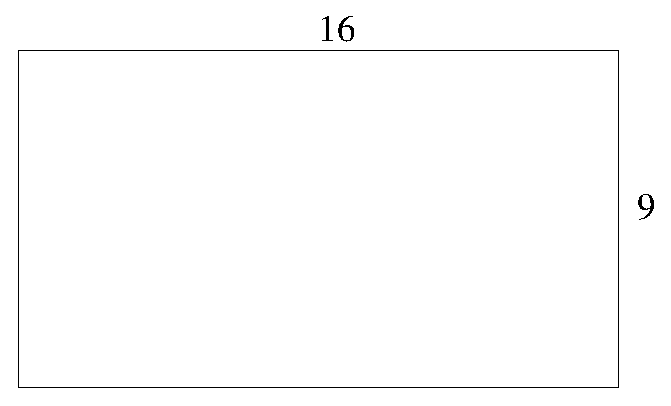
\includegraphics[scale=0.4]{Rect1}%
\lthtmlpictureZ
\lthtmlcheckvsize\clearpage}

{\newpage\clearpage
\lthtmlpictureA{tex2html_wrap1403}%
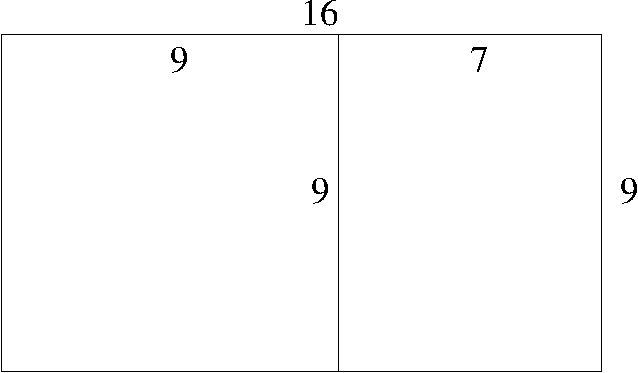
\includegraphics[scale=0.4]{Rect2}%
\lthtmlpictureZ
\lthtmlcheckvsize\clearpage}

{\newpage\clearpage
\lthtmldisplayA{displaymath539}%
\begin{displaymath}\frac{16}{9} = 1 + \frac{7}{9};\end{displaymath}%
\lthtmldisplayZ
\lthtmlcheckvsize\clearpage}

{\newpage\clearpage
\lthtmlinlinemathA{tex2html_wrap_inline653}%
$16/9$%
\lthtmlinlinemathZ
\lthtmlcheckvsize\clearpage}

{\newpage\clearpage
\lthtmlinlinemathA{tex2html_wrap_inline655}%
$7/9$%
\lthtmlinlinemathZ
\lthtmlcheckvsize\clearpage}

{\newpage\clearpage
\lthtmlinlinemathA{tex2html_wrap_inline659}%
$7$%
\lthtmlinlinemathZ
\lthtmlcheckvsize\clearpage}

{\newpage\clearpage
\lthtmlinlinemathA{tex2html_wrap_inline665}%
$2$%
\lthtmlinlinemathZ
\lthtmlcheckvsize\clearpage}

{\newpage\clearpage
\lthtmlpictureA{tex2html_wrap1412}%
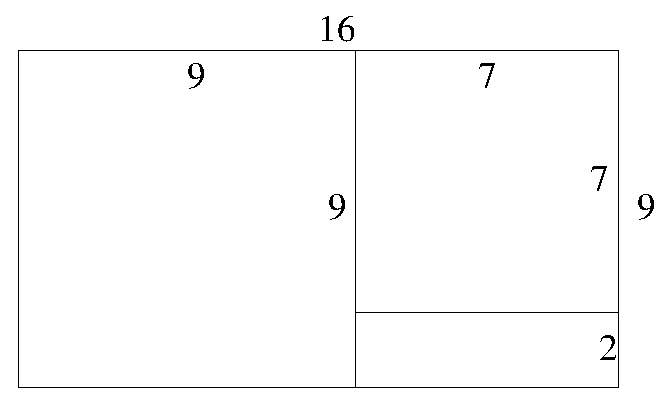
\includegraphics[scale=0.4]{Rect3}%
\lthtmlpictureZ
\lthtmlcheckvsize\clearpage}

{\newpage\clearpage
\lthtmldisplayA{eqnarraystar35}%
\begin{eqnarray*}
\frac{16}{9} &= &1 + \frac{7}{9} \\
&= &1 + \frac{1}{\displaystyle \frac{9}{7}} \\
&= &1 + \frac{1}{\displaystyle 1 + \frac{2}{7}}.
\end{eqnarray*}%
\lthtmldisplayZ
\lthtmlcheckvsize\clearpage}

{\newpage\clearpage
\lthtmlinlinemathA{tex2html_wrap_inline667}%
$1 + 1 + 3 + 2 = 7$%
\lthtmlinlinemathZ
\lthtmlcheckvsize\clearpage}

{\newpage\clearpage
\lthtmlpictureA{tex2html_wrap1418}%
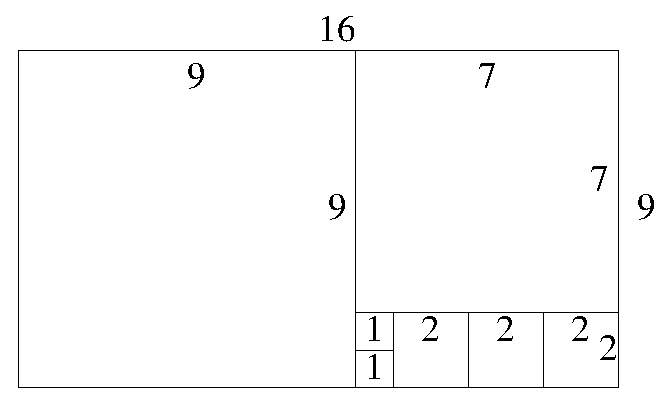
\includegraphics[scale=0.4]{Rect4}%
\lthtmlpictureZ
\lthtmlcheckvsize\clearpage}

{\newpage\clearpage
\lthtmldisplayA{displaymath540}%
\begin{displaymath}\frac{16}{9} = 1 + \frac{1}{\displaystyle 1 + \frac{1}{\displaystyle 3 + \frac{1}{2}}},\end{displaymath}%
\lthtmldisplayZ
\lthtmlcheckvsize\clearpage}

\stepcounter{section}
{\newpage\clearpage
\lthtmlfigureA{Def62}%
\begin{Def}{\rm Une \textit{fraction continue finie} est une expression de la forme suivante,
\begin{displaymath}a_0 + \frac{1}{\displaystyle a_1 + \frac{1}{\displaystyle a_1 + \frac{1}{\displaystyle a_2 + \cdots + \frac{1}{\displaystyle a_n}}}}\end{displaymath}
o� $n\ge 0$\  et $a_i\in\mathbb{R}$\  pour tout $0\le i\le n$.
\par
Si les $a_i\in\mathbb{Z}$\  pour tout $0\le i\le n$\  et $a_i>0$\  pour $0<i\le n$, alors la fraction continue est dite \textit{simple}.}
\end{Def}%
\lthtmlfigureZ
\lthtmlcheckvsize\clearpage}

{\newpage\clearpage
\lthtmlinlinemathA{tex2html_wrap_inline683}%
$[a_0,a_1,\cdots,a_n]$%
\lthtmlinlinemathZ
\lthtmlcheckvsize\clearpage}

{\newpage\clearpage
\lthtmlinlinemathA{tex2html_wrap_inline685}%
$a_i$%
\lthtmlinlinemathZ
\lthtmlcheckvsize\clearpage}

{\newpage\clearpage
\lthtmlinlinemathA{tex2html_wrap_inline687}%
$c_k = [a_0,a_1,\cdots,a_k]$%
\lthtmlinlinemathZ
\lthtmlcheckvsize\clearpage}

{\newpage\clearpage
\lthtmlinlinemathA{tex2html_wrap_inline689}%
$0\le k\le n$%
\lthtmlinlinemathZ
\lthtmlcheckvsize\clearpage}

{\newpage\clearpage
\lthtmlinlinemathA{tex2html_wrap_inline691}%
$24/13 = 1.84615...$%
\lthtmlinlinemathZ
\lthtmlcheckvsize\clearpage}

{\newpage\clearpage
\lthtmlinlinemathA{tex2html_wrap_inline693}%
$24$%
\lthtmlinlinemathZ
\lthtmlcheckvsize\clearpage}

{\newpage\clearpage
\lthtmlinlinemathA{tex2html_wrap_inline695}%
$13$%
\lthtmlinlinemathZ
\lthtmlcheckvsize\clearpage}

{\newpage\clearpage
\lthtmldisplayA{eqnarraystar75}%
\begin{eqnarray*}
24 &= &1\times 13 + 11 \\
13 &= &1\times 11 + 2 \\
11 &= &5\times 2 + 1 \\
2 &= &2\times 1 + 0,
\end{eqnarray*}%
\lthtmldisplayZ
\lthtmlcheckvsize\clearpage}

{\newpage\clearpage
\lthtmlinlinemathA{tex2html_wrap_inline697}%
$\pgcd(24,13) = 1$%
\lthtmlinlinemathZ
\lthtmlcheckvsize\clearpage}

{\newpage\clearpage
\lthtmlinlinemathA{tex2html_wrap_inline699}%
$24/13 = [1,1,5,2]$%
\lthtmlinlinemathZ
\lthtmlcheckvsize\clearpage}

{\newpage\clearpage
\lthtmldisplayA{eqnarraystar77}%
\begin{eqnarray*}
\frac{24}{13} &= &1 + \frac{11}{13} = 1 + \frac{1}{\displaystyle \frac{13}{11}} \\
&= &1 + \frac{1}{\displaystyle 1 + \frac{2}{11}} = 1 + \frac{1}{\displaystyle 1 + \frac{1}{\displaystyle \frac{11}{2}}} \\
&= &1 + \frac{1}{\displaystyle 1 + \frac{1}{\displaystyle 5 + \frac{1}{2}}}.
\end{eqnarray*}%
\lthtmldisplayZ
\lthtmlcheckvsize\clearpage}

{\newpage\clearpage
\lthtmlinlinemathA{tex2html_wrap_inline701}%
$10$%
\lthtmlinlinemathZ
\lthtmlcheckvsize\clearpage}

{\newpage\clearpage
\lthtmlinlinemathA{tex2html_wrap_inline703}%
$24/13$%
\lthtmlinlinemathZ
\lthtmlcheckvsize\clearpage}

{\newpage\clearpage
\lthtmlfigureA{Alg97}%
\begin{Alg}[Fractions continues]{
}{Soit $q\in\mathbb{Q}$, les quotients partiels de la fraction continue finie
\begin{displaymath}q = [a_0,a_1,\cdots,a_n]\end{displaymath}
peuvent �tre trouv�s gr�ce aux formules de r�currence suivantes
\begin{displaymath}\theta_k = \left\{
\begin{array}{ll}
q &\textrm{si }k = 0 \\
\frac{1}{\theta_{k-1} - a_{k-1}} &\textrm{si }0<k\le n
\end{array}
\right.\end{displaymath}
et
\begin{displaymath}a_k = \lfloor\theta_k\rfloor\end{displaymath}
avec $0\le k\le n$\  et $n$\  le plus petit naturel tel que $\theta_n = a_n$.}
\end{Alg}%
\lthtmlfigureZ
\lthtmlcheckvsize\clearpage}

{\newpage\clearpage
\lthtmlinlinemathA{tex2html_wrap_inline713}%
$\lfloor x\rfloor$%
\lthtmlinlinemathZ
\lthtmlcheckvsize\clearpage}

{\newpage\clearpage
\lthtmlinlinemathA{tex2html_wrap_inline715}%
$x\in\mathbb{R}$%
\lthtmlinlinemathZ
\lthtmlcheckvsize\clearpage}

{\newpage\clearpage
\lthtmlinlinemathA{tex2html_wrap_inline717}%
$x$%
\lthtmlinlinemathZ
\lthtmlcheckvsize\clearpage}

\stepcounter{section}
{\newpage\clearpage
\lthtmlfigureA{Pro111}%
\begin{Pro}
{Si on d�finit les entiers $p_0,p_1,\cdots,p_n$\  et $q_0,q_1,\cdots,q_n$\  par
\begin{displaymath}p_k = \left\{
\begin{array}{ll}
a_0 &\textrm{si }k = 0\\
a_0a_1 + 1 &\textrm{si }k = 1
\\a_kp_{k-1} + p_{k-2} &\textrm{si }2\le k\le n
\end{array}
\right.\end{displaymath}
et
\begin{displaymath}q_k = \left\{
\begin{array}{ll}
1 &\textrm{si }k = 0\\
a_1 &\textrm{si }k = 1
\\a_kq_{k-1} + q_{k-2} &\textrm{si }2\le k\le n
\end{array}
\right.,\end{displaymath}
alors on a
\begin{displaymath}c_k = \frac{p_k}{q_k}\end{displaymath}
pour $0\le k\le n$. De plus, on a
\begin{displaymath}p_kq_{k+1} - q_kp_{k+1} = (-1)^{k+1}\end{displaymath}
pour $0\le k\le n$. En particulier, on a $\pgcd(p_k,q_k) = 1$\  pour $0\le k\le n$.}
\end{Pro}%
\lthtmlfigureZ
\lthtmlcheckvsize\clearpage}

{\newpage\clearpage
\lthtmlinlinemathA{tex2html_wrap_inline731}%
$k = 0$%
\lthtmlinlinemathZ
\lthtmlcheckvsize\clearpage}

{\newpage\clearpage
\lthtmlinlinemathA{tex2html_wrap_inline733}%
$p_0/q_0 = a_0 = c_0$%
\lthtmlinlinemathZ
\lthtmlcheckvsize\clearpage}

{\newpage\clearpage
\lthtmlinlinemathA{tex2html_wrap_inline735}%
$k = 1$%
\lthtmlinlinemathZ
\lthtmlcheckvsize\clearpage}

{\newpage\clearpage
\lthtmlinlinemathA{tex2html_wrap_inline737}%
$p_1/q_1 = a_0 + 1/a_2 = c_1$%
\lthtmlinlinemathZ
\lthtmlcheckvsize\clearpage}

{\newpage\clearpage
\lthtmlinlinemathA{tex2html_wrap_inline739}%
$k$%
\lthtmlinlinemathZ
\lthtmlcheckvsize\clearpage}

{\newpage\clearpage
\lthtmlinlinemathA{tex2html_wrap_inline741}%
$k + 1$%
\lthtmlinlinemathZ
\lthtmlcheckvsize\clearpage}

{\newpage\clearpage
\lthtmldisplayA{eqnarraystar135}%
\begin{eqnarray*}
[a_0,a_1,\cdots,a_k,a_{k+1}] &= &\left[a_0,a_1,\cdots,a_k + \frac{1}{a_{k+1}}\right] \\
& = &\frac{\left(a_k + \frac{1}{a_{k+1}}\right)p_{k-1} + p_{k-2}}{\left(a_k + \frac{1}{a_{k+1}}\right)q_{k-1} + q_{k-2}} \\
&= &\frac{a_{k+1}(a_kp_{k-1} + p_{k-2}) + p_{k-1}}{a_{k+1}(a_kq_{k-1} + q_{k-2}) + q_{k-1}} \\
&= &\frac{a_{k+1}p_k + p_{k-1}}{a_{k+1}q_k + q_{k-1}},
\end{eqnarray*}%
\lthtmldisplayZ
\lthtmlcheckvsize\clearpage}

{\newpage\clearpage
\lthtmldisplayA{displaymath549}%
\begin{displaymath}p_0q_1 - q_0p_1 = -1.\end{displaymath}%
\lthtmldisplayZ
\lthtmlcheckvsize\clearpage}

{\newpage\clearpage
\lthtmldisplayA{eqnarraystar160}%
\begin{eqnarray*}
p_{k+1}q_{k+2} - q_{k+1}p_{k+2} &= &p_{k+1}(a_{k+2}q_{k+1} + q_k) - q_{k+1}(a_{k+2}p_{k+1} + p_k) \\
&= &-(p_kq_{k+1} - q_kp_{k+1}) \\
&= &(-1)^{k+2},
\end{eqnarray*}%
\lthtmldisplayZ
\lthtmlcheckvsize\clearpage}

{\newpage\clearpage
\lthtmlinlinemathA{tex2html_wrap_inline749}%
$d$%
\lthtmlinlinemathZ
\lthtmlcheckvsize\clearpage}

{\newpage\clearpage
\lthtmlinlinemathA{tex2html_wrap_inline751}%
$p_k$%
\lthtmlinlinemathZ
\lthtmlcheckvsize\clearpage}

{\newpage\clearpage
\lthtmlinlinemathA{tex2html_wrap_inline753}%
$q_k$%
\lthtmlinlinemathZ
\lthtmlcheckvsize\clearpage}

{\newpage\clearpage
\lthtmlinlinemathA{tex2html_wrap_inline757}%
$p_kq_{k+1} - q_kp_{k+1} = (-1)^{k+1}$%
\lthtmlinlinemathZ
\lthtmlcheckvsize\clearpage}

{\newpage\clearpage
\lthtmlinlinemathA{tex2html_wrap_inline759}%
$d = 1$%
\lthtmlinlinemathZ
\lthtmlcheckvsize\clearpage}

{\newpage\clearpage
\lthtmldisplayA{displaymath550}%
\begin{displaymath}c_0 = \frac{1}{1}, c_1 = \frac{2}{1}, c_2 = \frac{5\times 2 + 1}{5\times 1 + 1} = \frac{11}{6}\mbox{ et }c_3 = \frac{2\times 11 + 2}{2\times 6 + 1} = \frac{24}{13},\end{displaymath}%
\lthtmldisplayZ
\lthtmlcheckvsize\clearpage}

{\newpage\clearpage
\lthtmlinlinemathA{tex2html_wrap_inline763}%
$c_0 = 1$%
\lthtmlinlinemathZ
\lthtmlcheckvsize\clearpage}

{\newpage\clearpage
\lthtmlinlinemathA{tex2html_wrap_inline765}%
$c_1 = 2$%
\lthtmlinlinemathZ
\lthtmlcheckvsize\clearpage}

{\newpage\clearpage
\lthtmlinlinemathA{tex2html_wrap_inline767}%
$c_2 = 1.8333...$%
\lthtmlinlinemathZ
\lthtmlcheckvsize\clearpage}

{\newpage\clearpage
\lthtmlinlinemathA{tex2html_wrap_inline769}%
$c_3 = 1.84615...$%
\lthtmlinlinemathZ
\lthtmlcheckvsize\clearpage}

\stepcounter{section}
\stepcounter{subsection}
{\newpage\clearpage
\lthtmlfigureA{Pro194}%
\begin{Pro}{Si $(a_m)_{m\in\mathbb{N}}$\  est une suite d'entiers tels que $a_m>0$\  pour $m>0$, alors la suite $(c_m)_{m\in\mathbb{N}}$\  d�finie par
\begin{displaymath}c_m = \frac{p_m}{q_m} = [a_0,a_1,\cdots,a_m]\end{displaymath}
est convergente.}
\end{Pro}%
\lthtmlfigureZ
\lthtmlcheckvsize\clearpage}

{\newpage\clearpage
\lthtmlfigureA{Def200}%
\begin{Def}{\rm Soit $(a_m)_{m\in\mathbb{N}}$\  une suite d'entiers tels que $a_m>0$\  pour $m>0$, on appelle \textit{fraction continue infinie (simple)} toute expression de la forme
\begin{displaymath}\lim_{m\rightarrow\infty}[a_0,a_1,\cdots,a_m].\end{displaymath}
}
\end{Def}%
\lthtmlfigureZ
\lthtmlcheckvsize\clearpage}

{\newpage\clearpage
\lthtmlinlinemathA{tex2html_wrap_inline787}%
$[a_0,a_1,a_2,\cdots]$%
\lthtmlinlinemathZ
\lthtmlcheckvsize\clearpage}

{\newpage\clearpage
\lthtmlinlinemathA{tex2html_wrap_inline789}%
$a_m$%
\lthtmlinlinemathZ
\lthtmlcheckvsize\clearpage}

{\newpage\clearpage
\lthtmlinlinemathA{tex2html_wrap_inline791}%
$c_m = [a_0,a_1,\cdots,a_m]$%
\lthtmlinlinemathZ
\lthtmlcheckvsize\clearpage}

{\newpage\clearpage
\lthtmlinlinemathA{tex2html_wrap_inline793}%
$\sqrt{3}$%
\lthtmlinlinemathZ
\lthtmlcheckvsize\clearpage}

{\newpage\clearpage
\lthtmlinlinemathA{tex2html_wrap_inline797}%
$1$%
\lthtmlinlinemathZ
\lthtmlcheckvsize\clearpage}

{\newpage\clearpage
\lthtmldisplayA{eqnarraystar209}%
\begin{eqnarray*}
\sqrt{3} &= &\underbrace{\lfloor\sqrt{3}\rfloor}_{= 1}\times 1 + (\sqrt{3} - 1) \\
1 &= &\underbrace{\left\lfloor\frac{1}{\sqrt{3} - 1}\right\rfloor}_{= 1}\times(\sqrt{3} - 1) + \underbrace{(1 - 1\times(\sqrt{3} - 1))}_{= 2 - \sqrt{3}} \\
\sqrt{3} - 1 &= &\underbrace{\left\lfloor\frac{\sqrt{3} - 1}{2 - \sqrt{3}}\right\rfloor}_{= 2}\times(2 - \sqrt{3}) + \underbrace{(\sqrt{3} - 1 - 2\times(2 - \sqrt{3}))}_{= 3\sqrt{3} - 5} \\
2 - \sqrt{3} &= &\underbrace{\left\lfloor\frac{2 - \sqrt{3}}{3\sqrt{3} - 5}\right\rfloor}_{= 1}\times(3\sqrt{3} - 5) + \underbrace{(2 - \sqrt{3} - 1\times(3\sqrt{3} - 5))}_{7 - 4\sqrt{3}} \\
3\sqrt{3} - 5 &= &\underbrace{\left\lfloor\frac{3\sqrt{3} - 5}{7 - 4\sqrt{3}}\right\rfloor}_{= 2}\times(7 - 4\sqrt{3}) + (3\sqrt{3} - 5 - 2\times(7 - 4\sqrt{3})) \\
7 - 4\sqrt{3} &= &\cdots
\end{eqnarray*}%
\lthtmldisplayZ
\lthtmlcheckvsize\clearpage}

{\newpage\clearpage
\lthtmldisplayA{eqnarraystar245}%
\begin{eqnarray*}
\sqrt{3} &= &1 + \frac{1}{\displaystyle \frac{1}{\sqrt{3} - 1}} \\
&= &1 + \frac{1}{\displaystyle 1 + \frac{1}{\displaystyle \frac{\sqrt{3} - 1}{2 - \sqrt{3}}}} \\
&= &1 + \frac{1}{\displaystyle 1 + \frac{1}{\displaystyle 2 + \frac{1}{\displaystyle \frac{2 - \sqrt{3}}{3\sqrt{3} - 5}}}} \\
&= &1 + \frac{1}{\displaystyle 1 + \frac{1}{\displaystyle 2 + \frac{1}{\displaystyle 1 + \frac{1}{\displaystyle \frac{3\sqrt{3} - 5}{7 - 4\sqrt{3}}}}}} \\
&= &1 + \frac{1}{\displaystyle 1 + \frac{1}{\displaystyle 2 + \frac{1}{\displaystyle 1 + \frac{1}{\displaystyle 2 + \cdots}}}}.
\end{eqnarray*}%
\lthtmldisplayZ
\lthtmlcheckvsize\clearpage}

{\newpage\clearpage
\lthtmlinlinemathA{tex2html_wrap_inline799}%
$\sqrt{3} = [1,1,2,1,2,1,2,\cdots]$%
\lthtmlinlinemathZ
\lthtmlcheckvsize\clearpage}

{\newpage\clearpage
\lthtmlinlinemathA{tex2html_wrap_inline803}%
$1,2$%
\lthtmlinlinemathZ
\lthtmlcheckvsize\clearpage}

{\newpage\clearpage
\lthtmldisplayA{displaymath553}%
\begin{displaymath}\sqrt{3} = [1,\overline{1,2}].\end{displaymath}%
\lthtmldisplayZ
\lthtmlcheckvsize\clearpage}

{\newpage\clearpage
\lthtmlinlinemathA{tex2html_wrap_inline805}%
$\phi = (1 + \sqrt{5})/2$%
\lthtmlinlinemathZ
\lthtmlcheckvsize\clearpage}

{\newpage\clearpage
\lthtmldisplayA{displaymath554}%
\begin{displaymath}\phi = \frac{1 + \sqrt{5}}{2} = [1,\overline{1}].\end{displaymath}%
\lthtmldisplayZ
\lthtmlcheckvsize\clearpage}

{\newpage\clearpage
\lthtmlinlinemathA{tex2html_wrap_inline813}%
$\phi$%
\lthtmlinlinemathZ
\lthtmlcheckvsize\clearpage}

{\newpage\clearpage
\lthtmldisplayA{displaymath555}%
\begin{displaymath}p_k = 1,2,3,5,8,13,21,34,55,...\mbox{ et }q_k = 1,1,2,3,5,8,13,21,34,...,\end{displaymath}%
\lthtmldisplayZ
\lthtmlcheckvsize\clearpage}

{\newpage\clearpage
\lthtmlinlinemathA{tex2html_wrap_inline819}%
$x^2 - 3 = 0$%
\lthtmlinlinemathZ
\lthtmlcheckvsize\clearpage}

{\newpage\clearpage
\lthtmlinlinemathA{tex2html_wrap_inline823}%
$x^2 - x - 1 = 0$%
\lthtmlinlinemathZ
\lthtmlcheckvsize\clearpage}

\stepcounter{subsection}
{\newpage\clearpage
\lthtmlinlinemathA{tex2html_wrap_inline825}%
$\pi$%
\lthtmlinlinemathZ
\lthtmlcheckvsize\clearpage}

{\newpage\clearpage
\lthtmlinlinemathA{tex2html_wrap_inline829}%
$e$%
\lthtmlinlinemathZ
\lthtmlcheckvsize\clearpage}

{\newpage\clearpage
\lthtmldisplayA{displaymath556}%
\begin{displaymath}\pi = [3,7,15,1,292,1,\cdots],\end{displaymath}%
\lthtmldisplayZ
\lthtmlcheckvsize\clearpage}

{\newpage\clearpage
\lthtmldisplayA{displaymath557}%
\begin{displaymath}c_0 = \frac{3}{1},c_1 = \frac{22}{7},c_2 = \frac{333}{106},\cdots.\end{displaymath}%
\lthtmldisplayZ
\lthtmlcheckvsize\clearpage}

{\newpage\clearpage
\lthtmlinlinemathA{tex2html_wrap_inline833}%
$22/7$%
\lthtmlinlinemathZ
\lthtmlcheckvsize\clearpage}

{\newpage\clearpage
\lthtmlinlinemathA{tex2html_wrap_inline835}%
$333/106<\pi<22/7$%
\lthtmlinlinemathZ
\lthtmlcheckvsize\clearpage}

{\newpage\clearpage
\lthtmldisplayA{displaymath558}%
\begin{displaymath}e = [2,1,2,1,1,4,\cdots],\end{displaymath}%
\lthtmldisplayZ
\lthtmlcheckvsize\clearpage}

{\newpage\clearpage
\lthtmldisplayA{displaymath559}%
\begin{displaymath}c_0 = \frac{2}{1},c_1 = \frac{3}{1},c_2 = \frac{8}{3},c_3 = \frac{11}{4},\cdots.\end{displaymath}%
\lthtmldisplayZ
\lthtmlcheckvsize\clearpage}

\stepcounter{section}
\stepcounter{subsection}
{\newpage\clearpage
\lthtmlinlinemathA{tex2html_wrap_inline841}%
$x^2 - 2y^2 = 1$%
\lthtmlinlinemathZ
\lthtmlcheckvsize\clearpage}

{\newpage\clearpage
\lthtmlinlinemathA{tex2html_wrap_inline843}%
$\sqrt{2}$%
\lthtmlinlinemathZ
\lthtmlcheckvsize\clearpage}

{\newpage\clearpage
\lthtmlinlinemathA{tex2html_wrap_inline845}%
$(x_1,y_1),(x_2,y_2),\cdots$%
\lthtmlinlinemathZ
\lthtmlcheckvsize\clearpage}

{\newpage\clearpage
\lthtmlinlinemathA{tex2html_wrap_inline847}%
$x_i/y_i$%
\lthtmlinlinemathZ
\lthtmlcheckvsize\clearpage}

{\newpage\clearpage
\lthtmlinlinemathA{tex2html_wrap_inline851}%
$x_i^2 - 2y_i^2 = 1$%
\lthtmlinlinemathZ
\lthtmlcheckvsize\clearpage}

{\newpage\clearpage
\lthtmldisplayA{displaymath560}%
\begin{displaymath}\frac{x_i^2}{y_i^2} = 2 + \frac{1}{y_i^2}\rightarrow 2\end{displaymath}%
\lthtmldisplayZ
\lthtmlcheckvsize\clearpage}

{\newpage\clearpage
\lthtmlinlinemathA{tex2html_wrap_inline853}%
$y_i\rightarrow\infty$%
\lthtmlinlinemathZ
\lthtmlcheckvsize\clearpage}

{\newpage\clearpage
\lthtmlinlinemathA{tex2html_wrap_inline855}%
$(x_i,y_i)$%
\lthtmlinlinemathZ
\lthtmlcheckvsize\clearpage}

{\newpage\clearpage
\lthtmlinlinemathA{tex2html_wrap_inline857}%
$s_i$%
\lthtmlinlinemathZ
\lthtmlcheckvsize\clearpage}

{\newpage\clearpage
\lthtmlinlinemathA{tex2html_wrap_inline859}%
$d_i$%
\lthtmlinlinemathZ
\lthtmlcheckvsize\clearpage}

{\newpage\clearpage
\lthtmldisplayA{displaymath561}%
\begin{displaymath}s_1 = 2,s_{i+1} = d_i + s_i\end{displaymath}%
\lthtmldisplayZ
\lthtmlcheckvsize\clearpage}

{\newpage\clearpage
\lthtmldisplayA{displaymath562}%
\begin{displaymath}d_1 = 3,d_{i+1} = d_i + 2s_i.\end{displaymath}%
\lthtmldisplayZ
\lthtmlcheckvsize\clearpage}

{\newpage\clearpage
\lthtmlinlinemathA{tex2html_wrap_inline861}%
$(d_1,s_1),(d_3,s_3),(d_5,s_5),\cdots$%
\lthtmlinlinemathZ
\lthtmlcheckvsize\clearpage}

\stepcounter{subsection}
{\newpage\clearpage
\lthtmlinlinemathA{tex2html_wrap_inline867}%
$d\in\mathbb{N}$%
\lthtmlinlinemathZ
\lthtmlcheckvsize\clearpage}

{\newpage\clearpage
\lthtmldisplayA{displaymath563}%
\begin{displaymath}x = \frac{r^2 + d}{r^2 - d}\mbox{ et }y = \frac{2r}{r^2 - d}\end{displaymath}%
\lthtmldisplayZ
\lthtmlcheckvsize\clearpage}

{\newpage\clearpage
\lthtmlinlinemathA{tex2html_wrap_inline871}%
$r\in\mathbb{N}$%
\lthtmlinlinemathZ
\lthtmlcheckvsize\clearpage}

{\newpage\clearpage
\lthtmldisplayA{displaymath564}%
\begin{displaymath}\sqrt{d} = [a_0,\overline{a_1,\cdots,a_{n-1},2a_0}]\end{displaymath}%
\lthtmldisplayZ
\lthtmlcheckvsize\clearpage}

{\newpage\clearpage
\lthtmlinlinemathA{tex2html_wrap_inline873}%
$n\ge 1$%
\lthtmlinlinemathZ
\lthtmlcheckvsize\clearpage}

{\newpage\clearpage
\lthtmlinlinemathA{tex2html_wrap_inline877}%
$(p_{n-1},q_{n-1})$%
\lthtmlinlinemathZ
\lthtmlcheckvsize\clearpage}

{\newpage\clearpage
\lthtmlinlinemathA{tex2html_wrap_inline879}%
$n$%
\lthtmlinlinemathZ
\lthtmlcheckvsize\clearpage}

{\newpage\clearpage
\lthtmlinlinemathA{tex2html_wrap_inline881}%
$(p_{2n-1},q_{2n-1})$%
\lthtmlinlinemathZ
\lthtmlcheckvsize\clearpage}

{\newpage\clearpage
\lthtmldisplayA{displaymath565}%
\begin{displaymath}p_{kn-1}^2 - dq_{kn-1}^2 = (-1)^{kn}\end{displaymath}%
\lthtmldisplayZ
\lthtmlcheckvsize\clearpage}

{\newpage\clearpage
\lthtmlinlinemathA{tex2html_wrap_inline885}%
$k\ge 1$%
\lthtmlinlinemathZ
\lthtmlcheckvsize\clearpage}

{\newpage\clearpage
\lthtmlinlinemathA{tex2html_wrap_inline887}%
$r_{kn} = [2a_0,\overline{a_1,\cdots,a_{n-1},2a_0}]$%
\lthtmlinlinemathZ
\lthtmlcheckvsize\clearpage}

{\newpage\clearpage
\lthtmldisplayA{displaymath566}%
\begin{displaymath}\sqrt{d} = [a_0,a_1,\cdots,a_{kn-1},r_{kn}].\end{displaymath}%
\lthtmldisplayZ
\lthtmlcheckvsize\clearpage}

{\newpage\clearpage
\lthtmlinlinemathA{tex2html_wrap_inline889}%
$\sqrt{d}$%
\lthtmlinlinemathZ
\lthtmlcheckvsize\clearpage}

{\newpage\clearpage
\lthtmlinlinemathA{tex2html_wrap_inline891}%
$kn$%
\lthtmlinlinemathZ
\lthtmlcheckvsize\clearpage}

{\newpage\clearpage
\lthtmldisplayA{displaymath567}%
\begin{displaymath}\sqrt{d} = \frac{r_{kn}p_{kn-1} + p_{kn-2}}{r_{kn}q_{kn-1} + q_{kn-2}},\end{displaymath}%
\lthtmldisplayZ
\lthtmlcheckvsize\clearpage}

{\newpage\clearpage
\lthtmlinlinemathA{tex2html_wrap_inline893}%
$r_{kn} = a_0 + \sqrt{d}$%
\lthtmlinlinemathZ
\lthtmlcheckvsize\clearpage}

{\newpage\clearpage
\lthtmldisplayA{displaymath568}%
\begin{displaymath}\sqrt{d}(a_0q_{kn-1} + q_{kn-2} - p_{kn-1}) = a_0p_{kn-1} + p_{kn-2} - dq_{kn-1}.\end{displaymath}%
\lthtmldisplayZ
\lthtmlcheckvsize\clearpage}

{\newpage\clearpage
\lthtmldisplayA{displaymath569}%
\begin{displaymath}a_0q_{kn-1} + q_{kn-2} - p_{kn-1} = 0\mbox{ et }a_0p_{kn-1} + p_{kn-2} - dq_{kn-1} = 0,\end{displaymath}%
\lthtmldisplayZ
\lthtmlcheckvsize\clearpage}

{\newpage\clearpage
\lthtmlinlinemathA{tex2html_wrap_inline897}%
$p_{kn-1}$%
\lthtmlinlinemathZ
\lthtmlcheckvsize\clearpage}

{\newpage\clearpage
\lthtmlinlinemathA{tex2html_wrap_inline899}%
$-q_{kn-1}$%
\lthtmlinlinemathZ
\lthtmlcheckvsize\clearpage}

{\newpage\clearpage
\lthtmldisplayA{displaymath570}%
\begin{displaymath}p_{kn-1}^2 - dq_{kn-1}^2 = -(q_{kn-1}p_{kn-2} - p_{kn-1}q_{kn-2}) = (-1)^{kn}.\end{displaymath}%
\lthtmldisplayZ
\lthtmlcheckvsize\clearpage}

{\newpage\clearpage
\lthtmldisplayA{displaymath571}%
\begin{displaymath}p_{n-1}^2 - dq_{n-1}^2 = 1.\end{displaymath}%
\lthtmldisplayZ
\lthtmlcheckvsize\clearpage}

{\newpage\clearpage
\lthtmlinlinemathA{tex2html_wrap_inline905}%
$2n$%
\lthtmlinlinemathZ
\lthtmlcheckvsize\clearpage}

{\newpage\clearpage
\lthtmldisplayA{displaymath572}%
\begin{displaymath}p_{2n-1}^2 - dq_{2n-1}^2 = 1,\end{displaymath}%
\lthtmldisplayZ
\lthtmlcheckvsize\clearpage}

{\newpage\clearpage
\lthtmlinlinemathA{tex2html_wrap_inline907}%
$x^2 - 23y^2 = 1$%
\lthtmlinlinemathZ
\lthtmlcheckvsize\clearpage}

{\newpage\clearpage
\lthtmldisplayA{displaymath573}%
\begin{displaymath}\sqrt{23} = [4,\overline{1,3,1,8}],\end{displaymath}%
\lthtmldisplayZ
\lthtmlcheckvsize\clearpage}

{\newpage\clearpage
\lthtmlinlinemathA{tex2html_wrap_inline909}%
$n = 4$%
\lthtmlinlinemathZ
\lthtmlcheckvsize\clearpage}

{\newpage\clearpage
\lthtmlinlinemathA{tex2html_wrap_inline911}%
$(p_3,q_3) = (24,5)$%
\lthtmlinlinemathZ
\lthtmlcheckvsize\clearpage}

{\newpage\clearpage
\lthtmlinlinemathA{tex2html_wrap_inline913}%
$(x_1,y_1)$%
\lthtmlinlinemathZ
\lthtmlcheckvsize\clearpage}

{\newpage\clearpage
\lthtmlinlinemathA{tex2html_wrap_inline915}%
$(x_2,y_2)$%
\lthtmlinlinemathZ
\lthtmlcheckvsize\clearpage}

{\newpage\clearpage
\lthtmldisplayA{displaymath574}%
\begin{displaymath}(x_3,y_3) = (x_1x_2 + dy_1y_2,x_1y_2 + y_1x_2)\end{displaymath}%
\lthtmldisplayZ
\lthtmlcheckvsize\clearpage}

{\newpage\clearpage
\lthtmlinlinemathA{tex2html_wrap_inline917}%
$(24,5)$%
\lthtmlinlinemathZ
\lthtmlcheckvsize\clearpage}

{\newpage\clearpage
\lthtmldisplayA{displaymath575}%
\begin{displaymath}(24,5),(1151, 240),(55224, 11515),(2649601, 552480),\cdots.\end{displaymath}%
\lthtmldisplayZ
\lthtmlcheckvsize\clearpage}

\stepcounter{subsection}
{\newpage\clearpage
\lthtmlinlinemathA{tex2html_wrap_inline923}%
$22$%
\lthtmlinlinemathZ
\lthtmlcheckvsize\clearpage}

{\newpage\clearpage
\lthtmlinlinemathA{tex2html_wrap_inline925}%
$1773$%
\lthtmlinlinemathZ
\lthtmlcheckvsize\clearpage}

{\newpage\clearpage
\lthtmlinlinemathA{tex2html_wrap_inline929}%
$W$%
\lthtmlinlinemathZ
\lthtmlcheckvsize\clearpage}

{\newpage\clearpage
\lthtmlinlinemathA{tex2html_wrap_inline931}%
$X$%
\lthtmlinlinemathZ
\lthtmlcheckvsize\clearpage}

{\newpage\clearpage
\lthtmlinlinemathA{tex2html_wrap_inline933}%
$Y$%
\lthtmlinlinemathZ
\lthtmlcheckvsize\clearpage}

{\newpage\clearpage
\lthtmlinlinemathA{tex2html_wrap_inline935}%
$Z$%
\lthtmlinlinemathZ
\lthtmlcheckvsize\clearpage}

{\newpage\clearpage
\lthtmlinlinemathA{tex2html_wrap_inline937}%
$w$%
\lthtmlinlinemathZ
\lthtmlcheckvsize\clearpage}

{\newpage\clearpage
\lthtmlinlinemathA{tex2html_wrap_inline941}%
$y$%
\lthtmlinlinemathZ
\lthtmlcheckvsize\clearpage}

{\newpage\clearpage
\lthtmlinlinemathA{tex2html_wrap_inline943}%
$z$%
\lthtmlinlinemathZ
\lthtmlcheckvsize\clearpage}

{\newpage\clearpage
\lthtmldisplayA{eqnarraystar379}%
\begin{eqnarray*}
W = (1/2 + 1/3)X + Y &\mbox{ et } &X = (1/4 + 1/5)Z + Y, \\
Z = (1/6 + 1/7)W + Y &\mbox{ et } &w = (1/3 + 1/4)(X + x), \\
x = (1/4 + 1/5)(Z + z) &\mbox{ et } &z = (1/5 + 1/6)(Y + y), \\
y = (1/6 + 1/7)(W + w). & &
\end{eqnarray*}%
\lthtmldisplayZ
\lthtmlcheckvsize\clearpage}

{\newpage\clearpage
\lthtmlinlinemathA{tex2html_wrap_inline945}%
$W + X$%
\lthtmlinlinemathZ
\lthtmlcheckvsize\clearpage}

{\newpage\clearpage
\lthtmlinlinemathA{tex2html_wrap_inline947}%
$Y + Z$%
\lthtmlinlinemathZ
\lthtmlcheckvsize\clearpage}

{\newpage\clearpage
\lthtmlinlinemathA{tex2html_wrap_inline949}%
$z = 3515820v$%
\lthtmlinlinemathZ
\lthtmlcheckvsize\clearpage}

{\newpage\clearpage
\lthtmlinlinemathA{tex2html_wrap_inline951}%
$v\in\mathbb{N}$%
\lthtmlinlinemathZ
\lthtmlcheckvsize\clearpage}

{\newpage\clearpage
\lthtmldisplayA{displaymath576}%
\begin{displaymath}W = 10366482v, X = 7460514v, Y = 4149387v, Z = 7358060v,\end{displaymath}%
\lthtmldisplayZ
\lthtmlcheckvsize\clearpage}

{\newpage\clearpage
\lthtmldisplayA{displaymath577}%
\begin{displaymath}w = 7206360v, x = 4893246v, y = 5439213v, z = 3515820v.\end{displaymath}%
\lthtmldisplayZ
\lthtmlcheckvsize\clearpage}

{\newpage\clearpage
\lthtmlinlinemathA{tex2html_wrap_inline953}%
$50$%
\lthtmlinlinemathZ
\lthtmlcheckvsize\clearpage}

{\newpage\clearpage
\lthtmlinlinemathA{tex2html_wrap_inline955}%
$W + X = 17826996v$%
\lthtmlinlinemathZ
\lthtmlcheckvsize\clearpage}

{\newpage\clearpage
\lthtmldisplayA{displaymath578}%
\begin{displaymath}17826996 = 2^2\times 3\times 11\times 29\times 4657v,\end{displaymath}%
\lthtmldisplayZ
\lthtmlcheckvsize\clearpage}

{\newpage\clearpage
\lthtmlinlinemathA{tex2html_wrap_inline957}%
$v = 3\times 11\times 29\times 4657s^2 = 4456749s^2$%
\lthtmlinlinemathZ
\lthtmlcheckvsize\clearpage}

{\newpage\clearpage
\lthtmldisplayA{displaymath579}%
\begin{displaymath}W = 46200808287018s^2, X = 33249638308986s^2,\end{displaymath}%
\lthtmldisplayZ
\lthtmlcheckvsize\clearpage}

{\newpage\clearpage
\lthtmldisplayA{displaymath580}%
\begin{displaymath}Y = 18492776362863s^2, Z = 32793026546940s^2,\end{displaymath}%
\lthtmldisplayZ
\lthtmlcheckvsize\clearpage}

{\newpage\clearpage
\lthtmldisplayA{displaymath581}%
\begin{displaymath}w = 32116937723640s^2, x = 21807969217254s^2,\end{displaymath}%
\lthtmldisplayZ
\lthtmlcheckvsize\clearpage}

{\newpage\clearpage
\lthtmldisplayA{displaymath582}%
\begin{displaymath}y = 24241207098537s^2, z = 15669127269180s^2.\end{displaymath}%
\lthtmldisplayZ
\lthtmlcheckvsize\clearpage}

{\newpage\clearpage
\lthtmldisplayA{displaymath583}%
\begin{displaymath}Y + Z = 51285802909803s^2 = \frac{n(n + 1)}{2},\end{displaymath}%
\lthtmldisplayZ
\lthtmlcheckvsize\clearpage}

{\newpage\clearpage
\lthtmlinlinemathA{tex2html_wrap_inline961}%
$n\in\mathbb{N}$%
\lthtmlinlinemathZ
\lthtmlcheckvsize\clearpage}

{\newpage\clearpage
\lthtmlinlinemathA{tex2html_wrap_inline963}%
$8$%
\lthtmlinlinemathZ
\lthtmlcheckvsize\clearpage}

{\newpage\clearpage
\lthtmldisplayA{displaymath584}%
\begin{displaymath}410286423278424s^2 + 1 = (2n + 1)^2,\end{displaymath}%
\lthtmldisplayZ
\lthtmlcheckvsize\clearpage}

{\newpage\clearpage
\lthtmlinlinemathA{tex2html_wrap_inline967}%
$t = 2n + 1$%
\lthtmlinlinemathZ
\lthtmlcheckvsize\clearpage}

{\newpage\clearpage
\lthtmldisplayA{displaymath585}%
\begin{displaymath}t^2 - 410286423278424s^2 = 1,\end{displaymath}%
\lthtmldisplayZ
\lthtmlcheckvsize\clearpage}

{\newpage\clearpage
\lthtmldisplayA{displaymath586}%
\begin{displaymath}W + X + Y + Z + w + x + y + z = 776027140\cdots26719455081800,\end{displaymath}%
\lthtmldisplayZ
\lthtmlcheckvsize\clearpage}

{\newpage\clearpage
\lthtmlinlinemathA{tex2html_wrap_inline969}%
$200000$%
\lthtmlinlinemathZ
\lthtmlcheckvsize\clearpage}

{\newpage\clearpage
\lthtmlinlinemathA{tex2html_wrap_inline971}%
$206545$%
\lthtmlinlinemathZ
\lthtmlcheckvsize\clearpage}

{\newpage\clearpage
\lthtmlinlinemathA{tex2html_wrap_inline973}%
$80$%
\lthtmlinlinemathZ
\lthtmlcheckvsize\clearpage}

{\newpage\clearpage
\lthtmlinlinemathA{tex2html_wrap_inline975}%
$72$%
\lthtmlinlinemathZ
\lthtmlcheckvsize\clearpage}

{\newpage\clearpage
\lthtmlinlinemathA{tex2html_wrap_inline977}%
$35$%
\lthtmlinlinemathZ
\lthtmlcheckvsize\clearpage}

\stepcounter{section}
{\newpage\clearpage
\lthtmlfigureA{The392}%
\begin{The}{Si $q$\  est un nombre rationnel, alors il existe une fraction continue finie $[a_0,a_1,\cdots,a_n]$\  telle que
\begin{displaymath}q = [a_0,a_1,\cdots,a_n].\end{displaymath}
}
\end{The}%
\lthtmlfigureZ
\lthtmlcheckvsize\clearpage}

{\newpage\clearpage
\lthtmlfigureA{Lem395}%
\begin{Lem}{Soit $q = [a_0,a_1,\cdots,a_n]$\  une fraction continue finie. Si $c_{2k}$\  pour $0\le k\le \lfloor n/2\rfloor$\  et $c_{2k+1}$\  pour $0\le k\le (n-1)/2\rfloor$\   sont les convergents pairs et impairs respectivement, alors
\begin{enumerate}
\item
$c_0<c_2<c_4<\cdots$\  et $c_1>c_3>c_5>\cdots$.
\item
$c_{2k}<c_{2l+1}$\  pour $0\le k\le\lfloor n/2\rfloor$\  et $0\le l\le\lfloor (n - 1)/2\rfloor$.
\item
$q>c_{2k}$\  et $q<c_{2k+1}$\  pour $k\ge 0$\  et $q = c_{2l}$\  avec $n = 2l$\  si $n$\  est pair et $q = c_{2l+1}$\  avec $n = 2l + 1$\  si $n$\  est impair.
\end{enumerate}
}
\end{Lem}%
\lthtmlfigureZ
\lthtmlcheckvsize\clearpage}

{\newpage\clearpage
\lthtmlfigureA{Lem407}%
\begin{Lem}{Si $q = [a_0,a_1,\cdots,a_n]$\  est une fraction continue finie, alors on a
\begin{displaymath}\left|q - \frac{p_k}{q_k}\right| \le \frac{1}{q_kq_{k+1}}\end{displaymath}
pour tout $0\le k< n$.}
\end{Lem}%
\lthtmlfigureZ
\lthtmlcheckvsize\clearpage}

{\newpage\clearpage
\lthtmlfigureA{Pro419}%
\begin{Pro}{La valeur d'une fraction continue infinie est un nombre irrationnel.}
\end{Pro}%
\lthtmlfigureZ
\lthtmlcheckvsize\clearpage}

{\newpage\clearpage
\lthtmlfigureA{The422}%
\begin{The}{Pour tout nombre irrationnel $x$, il existe une fraction continue infinie $[a_0,a_1,\cdots]$\  telle que
\begin{displaymath}x = [a_0,a_1,\cdots].\end{displaymath}
}
\end{The}%
\lthtmlfigureZ
\lthtmlcheckvsize\clearpage}

{\newpage\clearpage
\lthtmlfigureA{The425}%
\begin{The}{Si la fraction continue de $\alpha\in\mathbb{R}$\  est p�riodique, alors $\alpha$\  est un irrationnel quadratique.}
\end{The}%
\lthtmlfigureZ
\lthtmlcheckvsize\clearpage}

{\newpage\clearpage
\lthtmlfigureA{The428}%
\begin{The}[Lagrange]{Si $\alpha\in\mathbb{R}$\  est un irrationnel quadratique, alors la fraction continue de $\alpha$\  est p�riodique.}
\end{The}%
\lthtmlfigureZ
\lthtmlcheckvsize\clearpage}

{\newpage\clearpage
\lthtmlfigureA{The431}%
\begin{The}{Si $d\in\mathbb{N}$\  n'est pas un carr� parfait, alors on a
\begin{displaymath}\sqrt{d} = [a_0,\overline{a_1,\cdots,a_{n-1},2a_0}]\end{displaymath}
pour $n\ge 1$.}
\end{The}%
\lthtmlfigureZ
\lthtmlcheckvsize\clearpage}


\end{document}
